% !TEX root=exama-221129-orap.tex
%--------------------------------------
% Create title frame
\titleframe

%--------------------------------------
% Table of contents
\begin{frame}{Overview}
  \setbeamertemplate{section in toc}[sections numbered]
  \tableofcontents[hideallsubsections]
\end{frame}


%==============================================
\section{ExaMA: Methods and Algorithms at Exascale}

\subsection{ExaMA}

\begin{frame}
  \frametitle{Objectives}

  \begin{center}
    Scale up methods and algorithms in predictive simulation data analysis, up to digital twinning, including uncertainty quantification and inverse problems

  \end{center}
  
\end{frame}

\subsection{Challenges}
\begin{frame}
  \frametitle{\insertsectionhead}
  \framesubtitle{\insertsubsectionhead}
  \footnotesize
  \begin{columns}
    \column{.5\textwidth}
    \begin{itemize}
      \item (C1) Reduce carbon (GHG) footprint in transportation, buildings, and cities
       \item (C2) Design, control, and manufacture of advanced materials
       \item (C3) Understand and simulate the human brain
       \item (C4) Understand fission and fusion reactions and design advanced experiment facilities for fusion
             \end{itemize} 
    \column{.5\textwidth}
    \begin{itemize}
      \item (C5) Monitor the health of our planet: climate prediction, impact assessment of environmental policies, rapid environmental hazards

        \item (C6) Monitor and personalize the health of human beings 
       \item (C7) Design drugs
       \item (C8) Design cost-effective renewable energy resources: batteries, biofuels, solar photovoltaics
       \item (C9) Understand the Universe
     \end{itemize} 
  \end{columns}

\end{frame}
\subsection{Bottlenecks}
\begin{frame}[fragile=singleslide]{\insertsectionhead}
  \framesubtitle{\insertsubsectionhead}
  \scriptsize
  \begin{columns}[]
    \begin{column}{.5\linewidth}
      \begin{itemize}
        \item (B1) Energy efficiency
        \item (B2) Interconnect Technology
        \item (B3) Memory technology
        \item (B4) Scalable systems software
        \item (B5) Programming systems
        \item (B6) Data Management
        \item (B7) Exascale Algorithms
      \end{itemize}
    \end{column}
    \begin{column}{.5\linewidth}
      \begin{itemize}
        \item (B8) Discovery, design, and decision algorithms
        \item (B9) Resilience, robustness and accuracy
        \item (B10) Scientific productivity
        \item (B11) Reproducibility, replicability of computation
        \item (B12) Pre/Post-processing
        \item (B13) Integrate Uncertainties
      \end{itemize}
    \end{column}
  \end{columns}
  \begin{alertblock}{Major Concerns}
    \footnotesize
    \begin{itemize}
      \item avoidance of communication  
      \item adaptive parallel grain and more compute-intensive at node level 
      \item handling of heterogeneous hardware and data representations and 
      \item self parametrization
    \end{itemize}
  \end{alertblock}
  
\end{frame}

\begin{frame}
  \frametitle{Exama is a Part of the NumPEx Software Stack}

  \begin{columns}[]
    \begin{column}{.5\linewidth}
      \begin{center}
        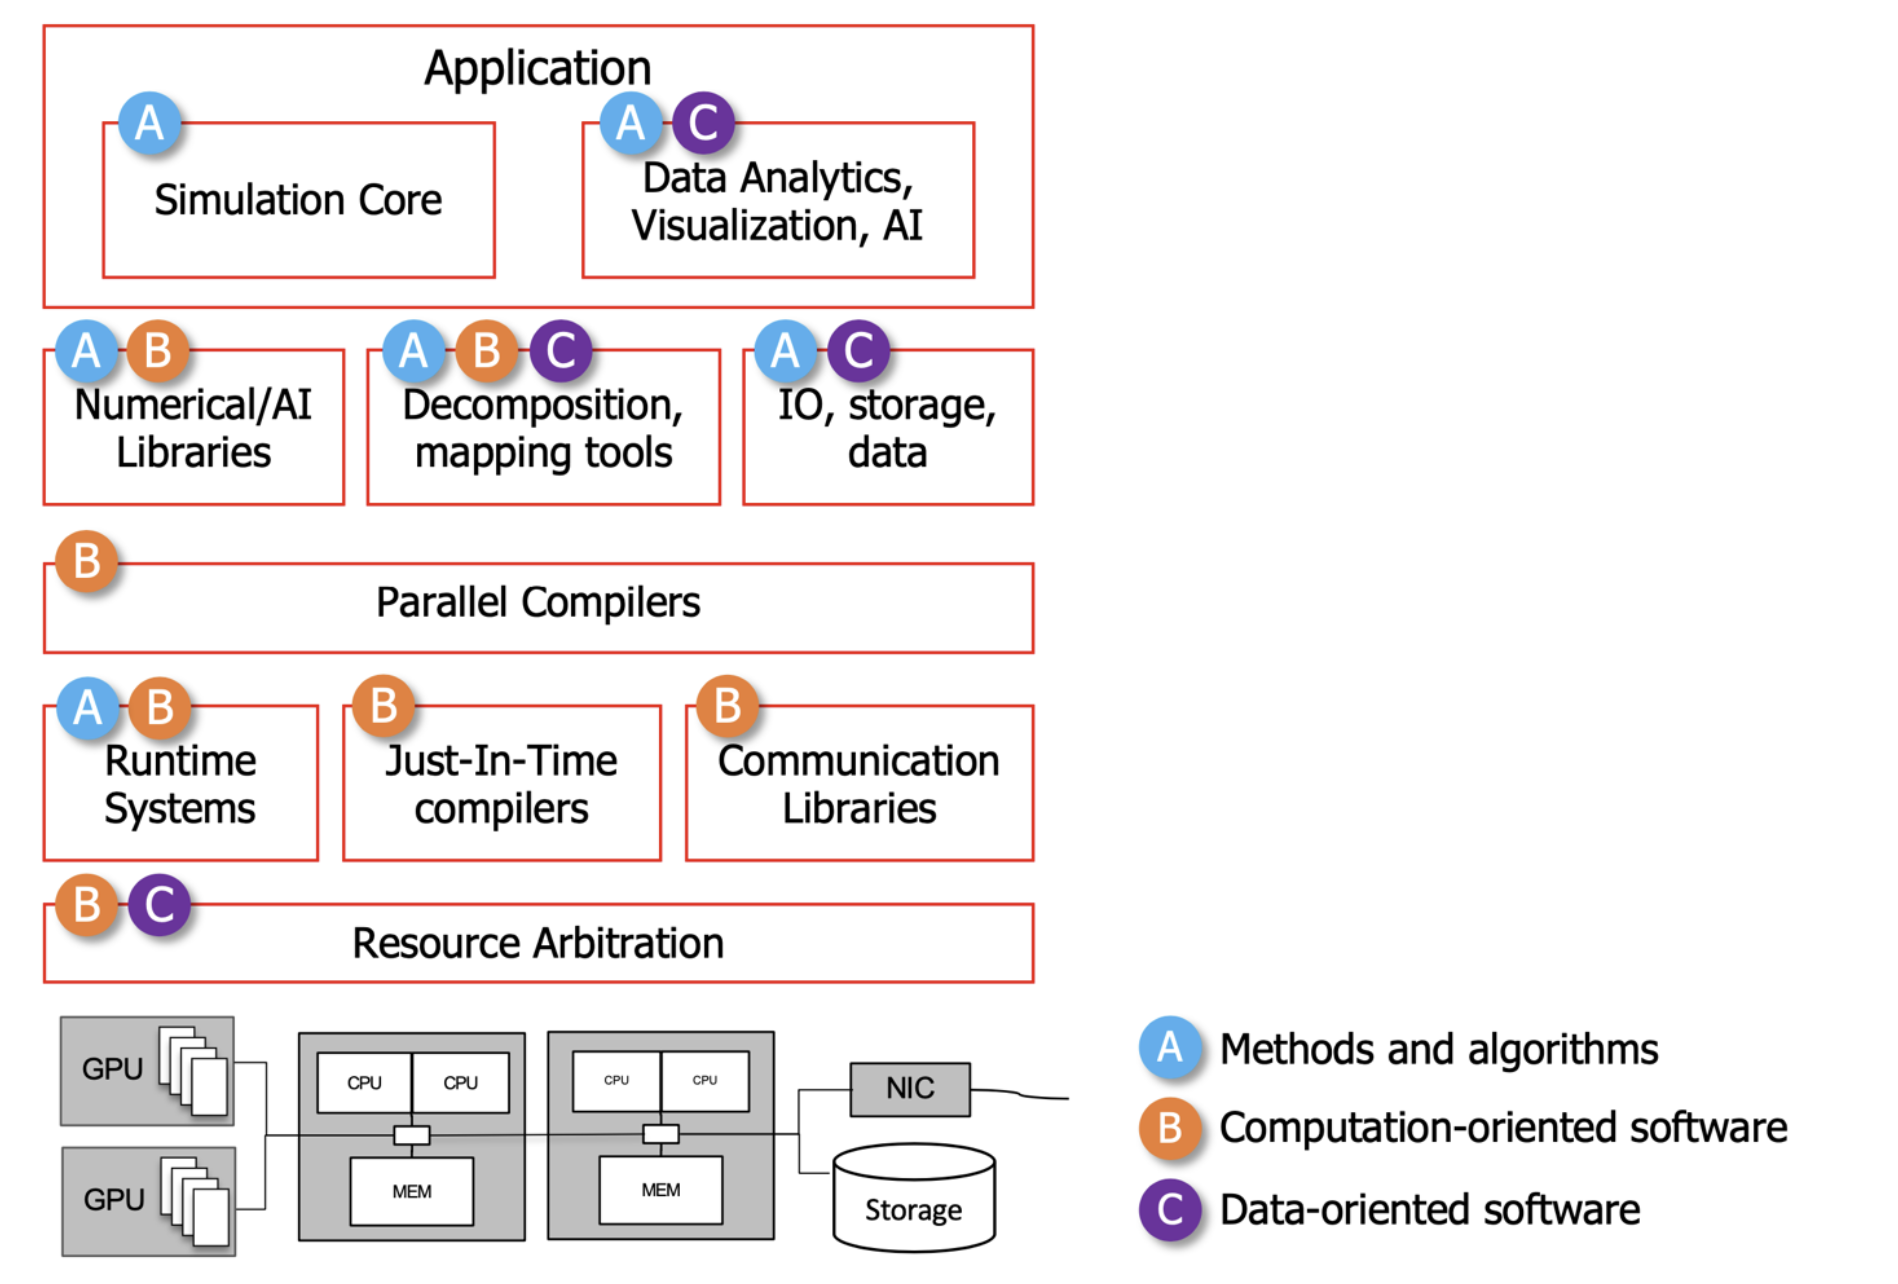
\includegraphics[height=.8\textheight]{../../figures/software-stack.png}  
      \end{center}
    \end{column}
    \begin{column}{.5\linewidth}
      Enable
      \begin{itemize}
        \item Performance and Scalability
        \item Productivity
        \item Reproducibility and reusability
        \item Efficiency, resilience, robustness
      \end{itemize}
    \end{column}
  \end{columns}
  
  
\end{frame}
\section{Work Packages}
\subsection{WP1: Modeling and Discretization}
\begin{frame}
  \frametitle{\insertsectionhead}
  \framesubtitle{\insertsubsectionhead}

  \begin{columns}
    \column{.5\textwidth}
    \begin{itemize}
      \item Geometric representation and their discrete counterparts [B2, B6, B7, B9, B11-B13] 
\
      \item physics-based models[B7, B10] 
    \end{itemize}
    \column{.5\textwidth}
  
  \begin{alertblock}{Data }
    Links with PC2-WP2/3, PC3-WP3 

  \end{alertblock}

  \end{columns}
\end{frame}


\subsection{WP2: Reduced order and AI driven methods for multi-fidelity modeling} 
\begin{frame}
  \frametitle{\insertsectionhead}
  \framesubtitle{\insertsubsectionhead}

  \begin{columns}
    \column{.5\textwidth}
    \begin{itemize}
      \item AI-driven, data-driven, reduced-order, and more generally surrogate models[B2, B7, B8, B10-B13]
      \item Multi-fidelity models [B2, B7, B8]
    \end{itemize}
    \column{.5\textwidth}
  
    \begin{alertblock}{Data}
    Contributors: SL, EF, HB, CP, JG\\
    Links with PC2-WP2/3, PC3-WP3
  \end{alertblock}

  \end{columns}
\end{frame}

\subsection{WP3: Linear, Multi-linear and Coupled Solvers at Exascale}
\begin{frame}
  \frametitle{\insertsectionhead}
  \framesubtitle{\insertsubsectionhead}
  \begin{columns}
    \column{.5\textwidth}
    \begin{itemize}
      \item Acceleration techniques for subspace-based methods [B1, B2, B5, B7, B9-B10].
      \item High dimensional problems [B1, B2, B5, B7, B10] 
      \item Randomization [B1, B2, B7, B10]
      \item Exploiting data-sparsity and multiple precision [B1, B2, B5, B7, B10]
      \item Adaptive solution strategies for exascale multiphysical and multiscale models [B7, B9-B11] 
    \end{itemize}
    \column{.5\textwidth}

    \begin{alertblock}{Data}
    Links with PC2-WP2/3   
  \end{alertblock}
  \end{columns}

\end{frame}

\subsection{WP4: Combine data and models, inverse problems at Exascale }
\begin{frame}
  \frametitle{\insertsectionhead}
  \framesubtitle{\insertsubsectionhead}
  \begin{columns}
    \column{.5\textwidth}
    [B2, B6, B7, B8, B13]
    \begin{itemize}
      \item Deterministic methods
      \item Stochastic methods
      \item Observations
      \item Taking advantage of multi-fidelity modeling
      \item challenges of multi-fidelity in inverse problems: criteria to update reduced models
    \end{itemize}
    \column{.5\textwidth}
    \begin{alertblock}{Data}
    Links with PC2-WP2/3,PC3-WP3
  \end{alertblock}
  \end{columns}
\end{frame}

\subsection{WP5: Optimize at Exascale }
\begin{frame}
  \frametitle{\insertsectionhead}
  \framesubtitle{\insertsubsectionhead}
  \begin{columns}
    \column{.5\textwidth}
    [B6-B8, B10, B13]
    \begin{itemize}
      \item Optimization 
      \begin{itemize}
        \item shape, dynamic shape optimization
        \item combinatorial optimization
        \item policy based optimization
        \item automated learning/AI for advanced design
      \end{itemize}
    \end{itemize}
    \column{.5\textwidth}
    \begin{alertblock}{data}
      Links with PC2-WP2/3,PC3-WP2 
    \end{alertblock}
  \end{columns}
\end{frame}

\subsection{WP6: Quantify uncertainty at Exascale - Links with P2-WP2/3,P3-WP2/3 }
\begin{frame}
  \frametitle{\insertsectionhead}
  \framesubtitle{\insertsubsectionhead}
  \begin{columns}
    \column{.5\textwidth}
    [B6-B8, B10, B13]
    \begin{itemize}
      \item Uncertainty quantification including 
      \begin{itemize}
        \item uncertainty propagation
        \item sensitivity analysis
        \item robust inversion
        \item UQ at different scales
        \item weak vs strong UQ
      \end{itemize}
    \end{itemize}
    \column{.5\textwidth}
    \begin{alertblock}{data}
      Links with PC2-WP2/3,PC3-WP2/3
    \end{alertblock}
  \end{columns}
\end{frame}

\subsection{WP7: Demonstrate methods and algorithms at Exascale}
\begin{frame}
  \frametitle{\insertsectionhead}
  \framesubtitle{\insertsubsectionhead}

  \begin{columns}
    \column{.5\textwidth}
    [B1-B13]
    \begin{itemize}
      \item Properties Verification on small/mini apps within PC1
      \item Co-design with the CDT and PC5
    \end{itemize}
    \column{.5\textwidth} 
    \begin{alertblock}{Data }
      Links with PC2-WP2/3,PC3-WP2/3 and PC5
    \end{alertblock}
   
  \end{columns}
\end{frame}

\subsection{Deliverables}

\begin{frame}
  \frametitle{\insertsectionhead}
  \framesubtitle{\insertsubsectionhead}
  \begin{itemize}
    \item  Methods, algorithms, and implementations that, taking advantage of the exascale architectures, empower modeling, solving, assimilating model and data, optimizing and quantifying uncertainty, at levels that are unreachable at present.
    \item Software libraries allowing to assemble specific critical reusable components, hiding the hardware complexity and exposing only the specific methodological interface
    \item Methodological and Algorithmic Patterns at exascale that can be reused efficiently in large scale applications (eg in weather forecasting)
    \item Enabling AI algorithms to attain performances at exascale, exploiting the methods (point 1) and the libraries (point 2) developed.
    \item \href{https://docs.google.com/document/d/1hjwSFRF63SyTUJJKGMNLHcJPr_S2JDHYXeBeQzHCSno/edit?usp=sharing}{\beamergotobutton{Demonstrators}}

  \end{itemize}


\end{frame}

\subsection{Milestones}

\begin{frame}
  \frametitle{\insertsectionhead}
  \framesubtitle{\insertsubsectionhead}

  \begin{itemize}
    \item   M1 Select IP-1 use-cases/demonstrators and associate methodology developments T0+6
    \item M2 benchmark IP-1 demonstrators on pre-exascale systems T0+9/T0+12
    \item M3 enable and benchmarks some new exascale  IP-1 components on pre-exascale/exascale systems T0+18, T0+36, T0+54, T0+60
\end{itemize}


\end{frame}




\section{Relations}

\subsection*{External Partner Status}
\begin{frame}
  \frametitle{\insertsectionhead}
  \framesubtitle{\insertsubsectionhead}

  Setting up this network and creating a group of external partners, we will succeed in
  \begin{itemize}
    \item bringing together our community to solve scientific challenges to move to the Exascale
    \item jointly develop software bricks to scale up to exascale
    \item creating/strengthening collaborations between external partners and Exa-MA partners via project co-leads, co-funding and/or use cases
    \item better structuring our community to respond effectively to European and international calls for projects.
  \end{itemize}

\end{frame}
\subsection{Entreprises}
\begin{frame}
  \frametitle{\insertsectionhead}
  \framesubtitle{\insertsubsectionhead}
  \begin{alertblock}{Entreprises}
    \begin{itemize}
      \item Expected: EDF, Safran, Total, Atos, Airbus
      \item Positive contact: Roche
    \end{itemize}
  \end{alertblock}
\end{frame}

\subsection{EPIC \& PEPR}
\begin{frame}
  \frametitle{\insertsectionhead}
  \framesubtitle{\insertsubsectionhead}
\begin{alertblock}{EPIC}
  \begin{itemize}
    \item Expected: Onera
    \item Others: Ifpen
  \end{itemize}
\end{alertblock}

\begin{alertblock}{PEPR}
  \begin{itemize}
    \item Expexted: IA
    \item Others: Diadem, TRACCS-Météo (in particular PC1-WP4)
  \end{itemize}
\end{alertblock}

\end{frame}

\subsection{Europe}
\begin{frame}
  \frametitle{\insertsectionhead}
  \framesubtitle{\insertsubsectionhead}
  \begin{alertblock}{CoE}
    \begin{itemize}
      \item Expected: Hidalgo2, Cheese-2P
      \item Others: CoE	EoCoE-3
    \end{itemize}
  \end{alertblock}

  \begin{alertblock}{Europe}
    \begin{itemize}
      \item Others: ERC-Synergy	EMC2, EuroHPC	Microcard, H2020 RIA Digital Twin	Bim2Twin,EuroHPC	European Master for HPC - EUMaster4HPC	
    \end{itemize}
  \end{alertblock}
\end{frame}

\section{Project Management}

\subsection{Principles}
\begin{frame}[fragile=singleslide]{\insertsectionhead}
  \framesubtitle{\insertsubsectionhead}

  \begin{itemize}
    \item \textbf{Openness} and \textbf{transparency} of the project 
    \item \textbf{Collaboration} with other projects : 
    \begin{itemize}
      \item 
        co-design with PC5, collaboration with PC2,3,4\
        \item 
          collaboration with other projects e.g. EuroHPC projects(Coe) and other PEPR (IA, Diademe,TRACCS-Météo...
    \end{itemize}
    \item \textbf{Inclusiveness} of the community 
    \begin{itemize}
      \item use the project as leverage for co-funding  or, also, collaborating outside the project eg phd co-advisors
      \item training : initial(train future PhD students) and continuous (broader community)
    \end{itemize}      
  \end{itemize}

\end{frame}


\begin{frame}
  \frametitle{}
  \framesubtitle{}

  \begin{center}
    \LARGE We are building the Exa-MA community 
  \end{center}
  Questions ?
  

\end{frame}

\appendix
\section{Appendix}
%==============================================
%==============================================
\subsection{NumPEx::PC1}
\begin{frame}{\insertsectionhead}
  \framesubtitle{ExaMA $\equiv$ PC1 $\equiv$ IP1}
  NUMPEX/ExaMa concentrates on the exascale aspects of the numerical methods, ensuring their scalability to existing and forthcoming hardware.
  \vfill
  Leaders: C Prud'homme \& H Barucq
  \begin{itemize}
    \item 5 Work packages
    \item wide range of topics: 
    \begin{itemize}
        \item Modeling and discretize
        \item Linear, multi-linear and coupled solvers at Exascale
        \item Combine data and  models at Exascale
        \item Optimize and quantify uncertainties at Exascale
    \end{itemize}
    \item Demonstrators through mini-apps will be used to verify the properties of the methods and algorithms developed.
  \end{itemize}
\end{frame}

\subsection{NumPEx::PC1 Team (a work still in progress)}

\begin{frame}
  \frametitle{\insertsectionhead}
  \framesubtitle{\insertsubsectionhead}

  Organismes financés
  \begin{itemize}
    \item CEA : DES(1 - 2), DAM (1)
    \item INRIA : Bordeaux(2-4),  Côte d'Azur (2), Grenoble(1), Lille(1), Paris(1)
    \item IPP (CMAP, Inria ASCII, Inria POEMS)
    \item UNISTRA  (IRMA-MOCO/Cemosis, Inria Tonus)
  \end{itemize}

  \begin{alertblock}{Other teams}
    \begin{itemize}
      \item Sorbonne Université ? (LJLL: Y  Maday, S Labbé; LIP6 Theo Marie, P Jolivet)
      \item ENS Lyon ? (Y Robert, ....) 
    \end{itemize}
  \end{alertblock}
\end{frame}

\subsection{Budget}

\begin{frame}
  \frametitle{\insertsectionhead}
  \framesubtitle{\insertsubsectionhead}
  \begin{itemize}
    \item si un universitaire est dans une equipe inria financée par Numpex, pas de souci
    \item Sinon comment collaborer (si necessaire)? Sur les sites, pourra t'on nous appuyer sur les conventions existantes pour 
    mettre en place des collaborations/des co-financements/..../co-directions/... ?
    \begin{itemize}
      \item Bordeaux: 
      \item Cotes d'Azur : 
      \item Grenoble : 
      \item Lille:  : 
      \item Paris : 
      \item Saclay : 
      \item Strasbourg : 
    \end{itemize}
  \end{itemize}
  \alert{Recemment accord cadre inria / cnrs signé}

\end{frame}

\section{Steering team}
\begin{frame}
  \frametitle{\insertsectionhead}
  \framesubtitle{\insertsubsectionhead}
\scriptsize
  \begin{itemize}
    \item CEA 
    \begin{itemize}
      \item DAM \textbf{Lydie Grospellier} (LGr)
      \item DES \textbf{Vincent Faucher} (VF) \textbf{Isabelle Ramière} (IR)  
    \end{itemize}
    \item INRIA 
    \begin{itemize}
      \item Bordeaux \textbf{Hélène Barucq} (HB) \textbf{Luc Giraud} (LGi)
      \item  Grenoble \textbf{Arthur Vidard} (AV)
      \item Lille \textbf{El-Ghazali Talbi} (ET) 
      \item Paris \textbf{Laura Grigori} (LG) \textbf{Frédéric Nataf} (FN)
      \item Sofia \textbf{Stephane Lanteri}(INRIA-Sofia) (SL) 
    \end{itemize}
    \item IPP \textbf{Josselin Garnier} \textbf{Marc Massot} (MM) \textbf{Loic Gouarin} (LGo)
    \item UPICARDIE \textbf{Mark Asch} (MA)
    \item UNISTRA \textbf{Christophe Prud'homme}(CP) \textbf{Emmanuel Franck} (EF) \textbf{Yannick Privat} (YP)
  \end{itemize}
  \alert{to be completed}
\end{frame}